
\chapter{Relatività Galileiana}

\section{Stato naturale di un corpo}

Secondo Aristotele, filosofo dell’antica Grecia,  lo stato naturale di un corpo è quello di quiete: se niente lo spingesse prima o poi si fermerebbe e così resterebbe in eterno. Siete d’accordo con lui? Sì? No? Provate a guardate, per esempio, il pallone fermo nel campo, la slitta carica di blocchi di marmo e l’acqua nel bicchiere. Tutto qui sulla terra sembra confermare le parole di Aristotele.

Purtroppo però quelle parole sono sbagliate: se la pensate come lui dovreste fare un upgrade di poco meno di 2 mila anni per  conoscere il genio toscano di Galileo Galilei il quale ci insegna che un corpo lasciato a sé stesso, cioè senza nessuna forza che agisca su esso, mantiene costante la propria velocità per sempre. Quindi, se nessuno lo spingesse più ed era fermo, fermo rimarrebbe proprio come sostiene Aristotele. Se però era in movimento continuerebbe a muoversi alla stessa velocità, senza accelerazioni o decelerazioni lungo una linea retta, per sempre. 

Questo tipo di moto, chiamato rettilineo uniforme, sembra quindi essere il vero stato naturale di un corpo. Sulla terra tutto sembra contraddire Galileo perché c’è sempre qualche agente frenante, cioè qualche forza che infine ferma la palla, la slitta o l'acqua nel bicchiere: ad esempio l’attrito dell’aria, della terra e la gravità stessa. Per avere un'immagine mentale a cui aggrapparvi pensate al meteorite nello spazio, lontano da qualsiasi pianeta: immaginatelo nel suo viaggio solitario, rettilineo e senza accelerazioni in eterno senza bisogno di nessuna forza che agisca su esso.

Newton ha saccheggiato questo principio importantissimo da Galileo e l'ha chiamato, assiomaticamente, \textit{primo principio della dinamica}, o semplicemente \textbf{principio d’inerzia}: ci ricorda come i corpi siano inerti, continuano a mantenere la velocità che avevano quando si smette di applicare loro una forza.


\section{Relatività galileiana, 1}

I due stati quindi, quello di quiete e quello di moto rettilineo uniforme, sono del tutto indistinguibili da un punto di vista fisico, e questo è il punto importante che apprenderemo adesso: se lanciate in alto una palla su un treno fermo vi ricadrà in mano, se fate lo stesso su un treno immaginario in moto rettilineo uniforme che viaggi a $200 km/h$ succederà la stessa identica cosa. Versate l’acqua nel bicchiere questa non scorre indietro per il fatto che il treno si muova ma continua a cadere perfettamente in verticale nel bicchiere come quando siete fermi.

Nulla tradisce lo stato di moto senza accelerazioni, nessun esperimento consente di distinguerlo dallo stato di quiete  e questo è una realtà di cui convincersi profondamente prima di affrontare la relatività di Einstein. Approfondiamo un poco l'argomento.

La palla è ferma in mano al viaggiatore, per lui non si muove, mentre la stessa palla, per una osservatrice ferma alla stazione si muove come il treno a $200 km/h$. La palla lanciata sul treno, dal fondo di un vagone verso la locomotiva viaggia a $30 km/h$ per i passeggeri del treno e a $230 km/h$ per la donna ferma alla stazione. Il calcolo è facile, basta sommare alla velocità della palla (per i passeggeri) quella del treno, $30+200=230$. 

Una palla lanciata invece nella direzione opposta viaggerà sempre a $30 km/h$ per i passeggeri ma a $170 km/h$ per la donna in stazione. In questo caso si sottraggono le velocità $200-30=170$.

La velocità è dunque un concetto relativo, come a dire che lo stato di quiete o di moto dipendono dall’osservatore e nessuno dei due sbaglia. 

Questo è il secondo punto da assimilare prima di procedere (il primo era l'indistinguibilità dei due stati di moto per chi li sperimenta). Se pensate che sia un ragionamento cervellotico questo della relatività, se non lo ritenete una realtà fisica vi sbagliate di grosso. Riflettete su questo: la palla lanciata delicatamente ($1 km/h$) tra due passeggeri del solito treno può anche essere presa al volo anche da un bambino piccolo, non gli procurerà alcun male. Un grosso male invece  sentirebbe quel bambino se  per lui la palla viaggiasse a $201 km/h$ orari, come ritiene la donna in stazione.

Rifletteteci sopra fino a domani, quando vi convincerete dello stato delle cose potrete procedere.

\section{Relatività galileiana, 2}

Se lo stato di quiete o di moto rettilineo uniforme sono indistinguibili da chi lo sperimenta allora abbiamo bisogno di un osservatore esterno per discriminare. La scelta dell’osservatore può portare a risultati diversi, come sappiamo: per qualcuno ci muoviamo, per altri stiamo fermi.

Senza osservatori esterni non esisterebbe neppure il concetto di moto. Non ci credete vero? Immaginate allora di essere soli nello spazio profondo, senza alcuna cosa attorno a voi: il moto esisterebbe? No, non esisterebbe senza un punto fisso, altro rispetto a noi. Se poi state pensando che anche in questo spazio potreste muovere le braccia vi invito a riflettere che muovere le braccia rispetto al corpo significa già avere un punto di riferimento: il corpo.

Per annullare completamente il concetto di moto dovete pensare ad un piccolissimo oggetto indivisibile senza nulla attorno: il concetto di movimento non esisterebbe proprio per questa minuscola pallina.

Prima di procedere dovete concordare sulla mia prossima affermazione: è la terra e muoversi attorno al sole. 

Il cardinale Bellarmino, che costrinse Galileo alla famosa abiura, non aveva torto da un punto di vista scientifico. Aveva invece torto da vendere imponendo con la violenza la visione di un Chiesa timorosa di perdere la propria egemonia. Si sbagliava anche sostenendo che Galileo avesse torto, la terra gira attorno al sole almeno quanto il sole giri attorno alla terra. Il moto è un concetto relativo.

Siete d’accordo? Se sì, procedete.


\section{Esperimento della pallina, 1}

In pochi paragrafi siamo quindi giunti attorno al 1600 apprendendo qualcosa del monumentale lavoro di Galileo: sappiamo che il moto, e quindi la velocità, sono concetti relativi. Anche la traiettoria lo è: la palla lanciata in verticale sul treno descrive una traiettoria dal basso verso l’alto e poi al contrario: una semiretta verticale per i passeggeri. Per la donna alla stazione però disegna una parabola, non ricade dove era stata lanciata perché il treno nel frattempo si è spostato in avanti a $200 km/h$.

Adesso dobbiamo formalizzare quando appreso in modo da passare da una descrizione della realtà, quella dei passeggeri, ad un'altra, quella della donna sulla pensilina. Lo faremo con un grafico molto semplice che useremo poi anche per descrivere la relatività di Einstein. Le due descrizioni della realtà si chiamano, tecnicamente, sistemi di riferimento\footnote{Ciascuno sistema di riferimento si muove rispetto all’altro in moto rettilineo uniforme a $200 km/h$ (la velocità del treno), si dicono perciò sistemi di riferimento inerziali e sono gli unici che studieremo.}  e servono per descrivere lo stesso evento in modi diversi: ogni evento avviene in una dato momento e in un punto preciso dello spazio per cui il sistema di riferimento della donna indicherà tempi e spazi con i simboli $(t,x)$ mentre quello dei passeggeri con i simboli $(t',x')$.

Vogliamo descrive nei due sistemi di riferimento lo stesso esperimento, visto da due punti di vista diversi: l'esperimento sarà tra i più stupidi mai escogitati, temo, e consisterà nel descrivere il moto di una pallina lanciata dall'ultimo vagone del treno contro la locomotiva. Ce la facciamo facile immaginando un treno formato da un solo vagone/locomotiva, senza ostacoli sulla strada della nostra pallina.

Diciamo poi il treno sia lungo  $c$, una distanza qualsiasi, ad esempio $20$ metri. Anzi, semplifichiamo ulteriormente diciamo che il treno è lungo $1$, un'unità di misura costruita apposta per noi, per cui $c=1$.  Inoltre diciamo che il treno si muova ad una velocità pari a $v$ che poniamo uguale a metà della sua lunghezza del treno $c/2$ (si legge $c$ mezzi).  Vuole dire che ogni secondo il nostro treno copre una distanza pari a metà della sua lunghezza, se fosse lungo $20$ metri ogni secondo ne percorrerebbe $10$ viaggiando quindi a $10$ metri al secondo, si indica così $v=10m/s$. Si dice che un'immagine valga cento parole per cui:

\begin{figure}[h!]
 \centering
 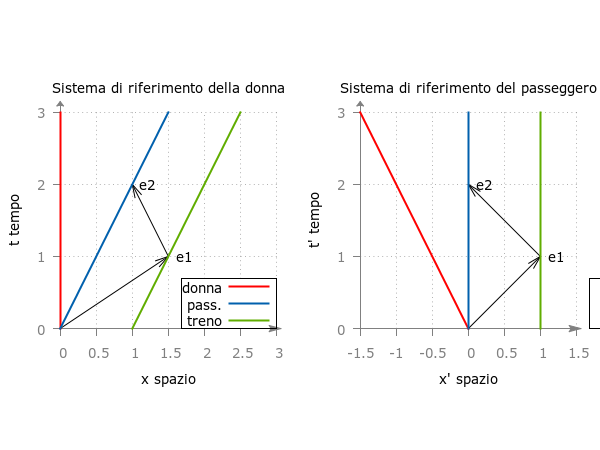
\includegraphics[scale=0.7]{figure/fig4}
 \caption{Esperimento della pallina}
\end{figure}

Non spaventatesi e continuate a leggere, iniziamo dal grafico di sinistra: rappresenta l'esperimento nel sistema di riferimento della signora. Dal suo punto di vista lei stessa è immobile, rimane sempre nella posizione $x=0$ per ogni tempo ed è quindi rappresentata dalla linea verticale rossa, quella più a sinistra. Nell'istante $0$ incrocia il passeggero seduto in coda al treno per cui, in quel momento, i due saranno entrambi nella posizione $0$ e poi il passeggero si allontana lungo la linea blu. La locomotiva del treno è sempre $c=1$ più avanti rispetto al passeggero perché il treno stesso è lungo $c$: la posizione della testa del treno è rappresentata dalla linea verde, quella più a destra.

Lo stesso esperimento è diverso invece per il passeggero, il cui sistema di riferimento è rappresentato nel grafico a destra. Dal suo punto di vista lui è quello fermo, indicato la linea centrale, sempre in blu. Anche la locomotiva per lui è ferma alla distanza $c$ da lui da cui la linea verde a destra. In questo sistema di riferimento si muove solo la signora e la pensilina su cui si trova: per il passeggero infatti la donna si allontana da lui a velocità $v$\footnote{Tecnicamente la velocità sarebbe $-v$, dove il segno meno indica che la donna si muove nella direzione opposta al treno.} come vediamo nella linea rossa a sinistra.

Riepilogando: la linea rossa, che si chiama linea di universo, rappresenta la donna, mentre il treno si estende dalla linea blu, la coda, a quella verde, la locomotiva.

Soffermatevi il tempo necessario per comprendere questi grafici in cui troviamo rappresentati i concetti fino a qui espressi a parole.

\section{Esperimento della pallina, 2}

Pronti a riprendere il nostro esperimento? Bene, diciamo che quando la coda del treno passa davanti alla donna alla stazione, il passeggero seduto proprio in fondo al treno lancia la palla nella direzione di marcia: ci chiediamo quando la palla tocchi la testa del treno? Quando rimbalzando indietro torna in mano al passeggero? E soprattutto: per i due sistemi di riferimento, quello della donna e quello del passeggero, come saranno diversi questi calcoli?

Ci manca un dato? Sì, sappiamo che il treno è lungo $c=1$ e che viaggia a $v=c/2$ ma a quando viaggia la pallina per il passeggero sul treno? Diciamo, sempre per facilitarci il lavoro, $c=1$: cioè ogni secondo la pallina percorre la lunghezza del treno (sì,viaggia parecchio veloce questa pallina).

Abbiamo promesso di usare solo le quattro operazioni e così faremo: con dati così semplici il calcolo è davvero facile. Per il passeggero seduto in fondo al treno la palla, che ogni secondo percorre $c$, ci mette quindi un solo secondo a raggiungere la locomotiva distante $c$.  Un secondo per andare e un altro secondo per tornare indietro.

Possiamo vederlo bene nella figura 1, grafico di destra: la freccia che esce dall'origine rappresenta il percorso della pallina che dopo $1$ secondo raggiunge la testa del treno rappresentata dalla linea verde. Possiamo chiamare questo evento $e1$ intendendo sia  quando ($1$ secondo) sia dove (posizione $c$) la pallina incontra la locomotiva. Il viaggio di ritorno della pallina è rappresentato dalla seconda freccia che da $e1$ torna verso il passeggero, linea blu, intercettandolo dopo $1$ secondo. Quel momento e quel luogo lo chiamiamo evento $e2$.

Lo stesso esperimento è descritto in modo molto diverso dalla signora sulla pensilina: per lei la testa del treno si sposta ad una velocità pari a $v=c/2$, linea verde del grafico a sinistra, per cui la pallina dovrà rincorrerla. Per la signora la pallina si muove ad una velocità pari a $c+v$, per quanto abbiamo detto nei paragrafi precedenti. 

Quanto ci mette a raggiungere la testa del treno?  Che domanda scontata direte voi, non serve nemmeno fare i calcoli: se quando la pallina tocca la testa del treno l’orologio del passeggero segna $1$ secondo, anche quello della donna, per lo stesso evento $e1$, dovrà segnare lo stesso tempo. Per cui la pallina tocca la locomotiva dopo $1$ secondo. 

Avete ragione... ma solo per ora come vedremo più avanti. In ogni caso per velocità così ridotte anche per la donna la pallina ci mette un secondo a raggiungere la testa del treno e uno a tornare indietro. Il percorso della pallina è rappresentato anche qui dalle due frecce nel grafico a sinistra. 

Se però i due sistemi di riferimento concordano sui tempi non concordano però sulle velocità o sullo spazio percorso: riassumiamo nella prossima tabella i nostri risultati.

\begin{center}
\begin{tabular}{>{\itshape}l >{\itshape}c >{\itshape}c }
\toprule
            & \textbf{donna} & \textbf{passeggero} \\
velocità treno            & $v$   & $0$  \\ 
velocità pensilina        & $0$   & $-v$  \\
velocità pallina          & $c+v$ & $c$  \\
secondi dell'esperimento  & $2$   & $2$  \\
distanza percorsa dalla pallina   & $2v$  & $2c$  \\
lunghezza del treno       & $c$   & $c$  \\
\bottomrule
\end{tabular} 
\end{center}


Nei due sistemi di riferimento la velocità relativa di treni e pensilina coincide, $v$. Anche i tempi coincidono, ma non la velocità della pallina: misurandola con qualsiasi mezzo per la donna sarebbe maggiore che per il passeggero. Quindi se la velocità è maggiore, ma i tempi sono li stessi tempi, se ne deduce che la pallina ha percorso un tragitto più lungo per il donna rispetto a quanto creda il passeggero.

Facciamo un ultimo sforzo per verificare la lunghezza del treno per la donna sulla pensilina: sappiamo che dopo $1$ secondo la locomotiva  si trova alla distanza $v+c$. La parte coda del treno invece si trova, dopo $1$ secondo, alla distanza $v$. Quindi otteniamo che il treno sia lungo $c$ e tutto quadra.

Rifletteteci un po’ sopra prima di procedere. Se vi va e vi ricordate la semplice algebra della terza media  saltate  all’appendice per provare a rifare i calcoli assieme.


\section{Relatività galileiana, 3}

Questo è un paragrafo di tutto relax: faremo solo dei disegnini per rappresentare l’esperimento visto in precedenza e passare da un sistema di riferimento ad un altro, senza fare calcoli ma limitandosi a guardare.

Ritroviamo in entrambi i grafici gli eventi $e1$, la pallina raggiunge la locomotiva e $e2$, quando questa torna in mano al passeggero. Le frecce qui non rappresentano più il percorso della pallina ma ci mostrano come, dato un evento, se ne possano trovare le coordinate cioè quando accade e dove accade. A sinistra abbiamo la condizione usuale, quella imparata a scuola, per cui dall'evento scendiamo in verticale per trovare la posizione, $x=1.5$, oppure in orizzontale per ottenere il tempo $t=1$. In pratica muoviamo dall'evento agli assi cartesiani (in blu nel grafico).

\begin{figure}[h!]
 \centering
 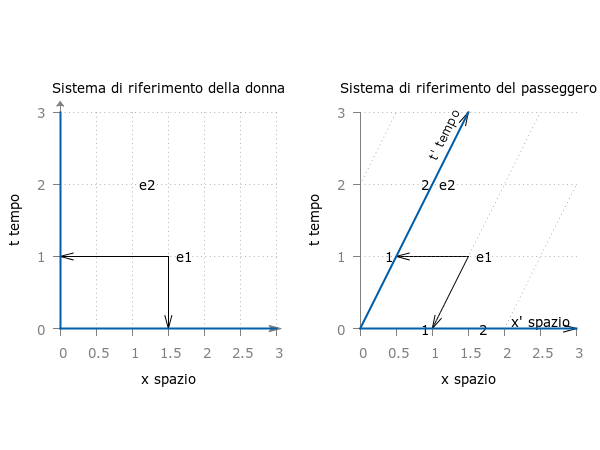
\includegraphics[scale=0.7]{figure/fig5}
 \caption{relatività galileiana}
\end{figure}

Per ottenere le coordinate $x'$ e $t'$ dello stesso evento $e1$ dal punto di vista del passeggero si possono tenere fermi i punti degli eventi però utilizzando degli assi diversi, visibili sempre in blu nel grafico di destra. Anche in questo caso ci muoviamo dall'evento $e1$ verso gli assi e leggiamo lì sopra le coordinate $x'=1$ e $t'=1$.

Useremo queste rappresentazioni per avere sott'occhio contemporaneamente i due sistemi di riferimento in un solo grafico e semplificarci i ragionamenti. \footnote{Il sistema di assi di destra chiaramente non è cartesiano perché gli assi non sono tra loro ortogonali. C'è però di peggio: la distanza dall'origine per l'asse $t'$ non riporta il tempo ma una sua funzione lineare, $t'\sqrt{1+v^2}$. Non ci cureremo troppo di questi dettagli limitandoci a leggere le etichette sui nuovi assi obliqui senza chiederci come si misurino.}

Provate da soli a riportare nel grafico a sinistra gli assi $x'$ e $t'$ in modo da avere in un solo colpo d'occhio entrambi i sistemi di riferimento.

\section{Sincronizzare gli orologi}

Ovvero come misurare gli intervalli di tempo. Con un cronometro rispondete? Be’, certo. Però dovremo domandarci come faccia il passeggero, seduto a metà treno, a sapere che esattamente dopo un $1$ la pallina tocca la testa del treno? Lui si trova da un’altra parte in quel momento quindi come può esserne certo?

Pensate ad un modo sicuro per riuscirci, anche se stravagante, non importa.

Pensato?

Si potrebbe fare così: nel momento in cui incrocia la donna sulla banchina il passeggero potrebbe sincronizzare due orologi con quello di lei e poi, successivamente, potrebbe andare a mettere uno dei due nella testa del treno. A quel punto ritorna al suo posto, lancia la palla e quando questa colpisce la testa del treno scatta una foto o guarda direttamente con un binocolo l’orologio in modo da sapere con esattezza l’orario in quel momento. La stessa cosa può fare anche la donna sincronizzando orologi quando incroci il passeggero e poi piazzarli lungo il binario per poi guardare quello vicino al luogo in cui la palla raggiungerà la testa del treno. Oppure anche qui fare delle foto dei vari eventi. 

Esiste però un modo più generale per sincronizzare gli orologi che evita di spostarli \footnote{Come scopriremo spostare i orologi sincronizzati significa... che non sono più sincronizzati!}: prima si dispongono dove si crede, a metà treno, sulla locomotiva, sulla pensilina, ovunque insomma. Poi quando il passeggero incroci la donna ferma alla stazione si azzerano gli orologi che hanno in mano e contemporaneamente si lancia un raggio di luce verso gli altri orologi. Dal momento che la velocità della luce è \textit{tragicamente} costante, conoscendo la distanza degli orologi, si sa esattamente dopo quanti secondi saranno raggiunti dal raggio e in quel momento inizieranno a muoversi. Non è difficile: diciamo che la luce percorra una distanza pari a $c$ ogni secondo. L'orologio che si trovi alla distanza $c$ dal passeggero sarà raggiunto dopo $1$ secondo e in quel momento segnerà $1$ e inizierà a contare il tempo. L'orologio che si trovi alla distanza $2c$ dal passeggero sarà raggiunto dopo $2$ secondo e in quel momento segnerà $2$ e inizierà a contare il tempo.  

Semplice no? Questo modo di sincronizzare gli orologi tra l'altro è l'unico possibile sulle grandi distanze, tipo quelle interplanetarie. 

Ricapitolando, una volta sincronizzati gli orologi segneranno tutti la stessa ora. Ora questo paragrafo vi sembrerà ovvio, ma sono pronto a scommettere che ci tornerete sopra quando nella prossima sezione discuteremo la relatività del tempo.


\section{Misurare le lunghezze}

Per misurare la lunghezza di un oggetto come si procede? Si pone un capo del metro su un lato, l'altro capo dalla parte opposta e si legge la lunghezza. Da notare come questa questa operazione deve essere simultanea: se quando leggo la misura su un capo l'altro non coincide più con l'estremità dell'oggetto da misurare non sto facendo un buon lavoro. 

\begin{figure}[h!]
 \centering
 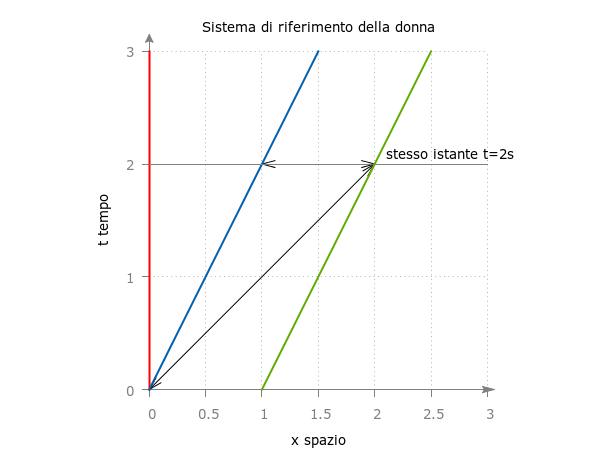
\includegraphics[scale=0.7]{figure/fig7}
 \caption{relatività galileiana}
\end{figure}


Quest'ultima informazione è importante anche se non ora non ci sembra: il fatto che le distanze tra i due estremi dell'oggetto debbano essere misurate \textit{simultaneamente}, nello stesso istante, ci procurerà qualche problema nei prossimi paragrafi. Nella figura 3 si vede chiaramente che misurando in istanti diversi (la linea obliqua nera) si ottiene una lunghezza diversa rispetto a misurare nello stesso istante (linea orizzontale nera): la lunghezza del treno risulterebbe maggiore di $1$ considerando gli estremi in momenti diversi. 

Infine, sapete immaginare un metodo più generale per misurare le distanze? Per oggetti lunghissimo o lontani da noi? No? Non avete letto bene il paragrafo precedente bene allora. Tornate indietro?

Usando la luce? Esatto: si lanciano due raggi in modo che raggiungano \textbf{contemporaneamente} gli estremi dell'oggetto e poi si aspetta che ritornino indietro. Vediamo un grafico per capire meglio la situazione:

FIG MISURARE LUNGHEZZE

Oh bene, a questo punto disponiamo di tutti gli elementi per comprendere facilmente la teoria della relatività speciale di  Einstein. Partiamo!
